
The purpose of this experiment is to determine the speed of light by employing a Foucault rotating-mirror setup. A laser beam is directed onto a rapidly spinning mirror, then reflected toward a concave mirror and back. Because light requires a finite time to travel, any increase in the rotating mirror’s angular velocity causes a small lateral shift of the returning beam, which is observable in the microscope’s field of view. By systematically varying the mirror’s rotation speed and measuring the corresponding spot displacement, it becomes possible to calculate the speed of light from macroscopic, measurable quantities such as the rotation frequency, the geometrical distances along the optical bench (\(D, a, f_2\)), and the shift observed in the microscope. The precise alignment of the beam and mirrors is crucial, so considerable attention is given to centering the laser beam on each element and ensuring the return beam follows the same path. 


The data collection includes several measurements of the spot’s displacement  \(\Delta\delta\) at different rotational frequencies in both clockwise and counterclockwise directions, as well as transitions from maximum speed in one direction to maximum speed in the other. This set of measurements, along with the known distances and lens focal lengths, allows for calculating the speed of light and estimating uncertainties arising from micrometer resolution, alignment accuracy, and possible variations in the mirror’s angular velocity.


\begin{figure}[h]
    \centering
    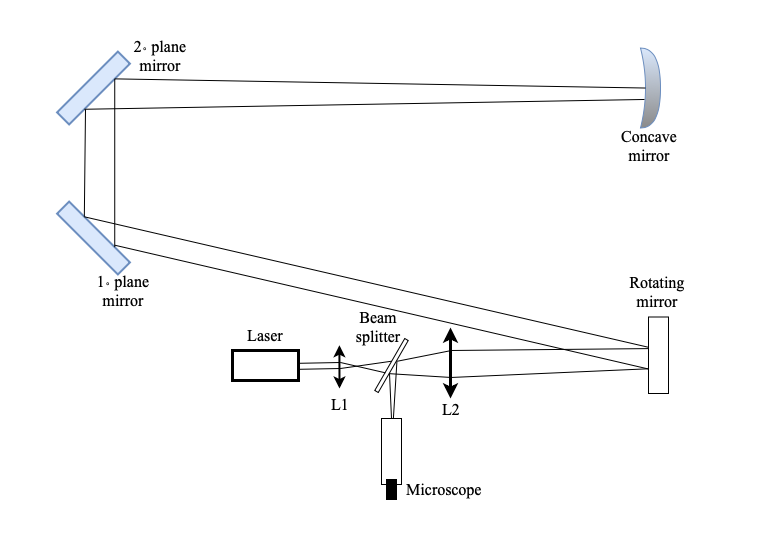
\includegraphics[width=\linewidth]{LightSpeed/image123.png}
    \caption{Foucault device used in the laboratory experiment}
    \label{fig:foucault}
\end{figure}
